\chapter{Vergleich der Browser}
\label{chapter:vergleich-der-browser}

- Zusammenfassung: Vergleich Tor v. Firefox und Brave v. Chrome

\subsection*{Common Locations}
- Process Monitor Logfiles: 
	> Keine PB Artefakte bei beiden Browsern
	> Abbildung Anzahl Schreiboperationen pro Browser
- SQLite Datenbänke
	> Keine PB Artefakte in SQLite Datenbänken beider Browser
	> Gleiche Datenbänke: Evtl. hervorheben, bei welchen Browser mehr geschrieben wurde, ODER: Diagramm mit Anazhl Schreiboperationen pro SQLite DB verglichen zwischen Browsern
		(Gestacktes Balkendiagramm zu veränderten SQLite DBs => Erst bei Vergleich mit Tor!)

\subsection*{Registry}
 "Sessionstore-Backup" fehlt in Tor

TODO: Kreisdiagramme/Balkendiagramme mit Gesamtzahl an (Non-)Firefox Yarascan-Treffer erst im Vergleich mit Tor
- Firefox v. Chrome ("Standardbrowser")
- Tor v. Brave ("Sichere Browser")
- Zum Schluss: "Eine große Tabelle" mit den wichtigsten Kategorien?

\subsection*{Uncommon Locations}
- Autopsy Stichwortsuche: keine Suchergebnisse bei beiden Browsern
- Autopsy Kategorien: keine PB Artefakten in kategorisierten Dateien, evtl. unterschiedlich Kategorisierte Dateien hervorheben
- Volatility Artefakte:

\begin{table}[h!]
	\resizebox{\linewidth}{!}{
	\begin{tabular}{r}
		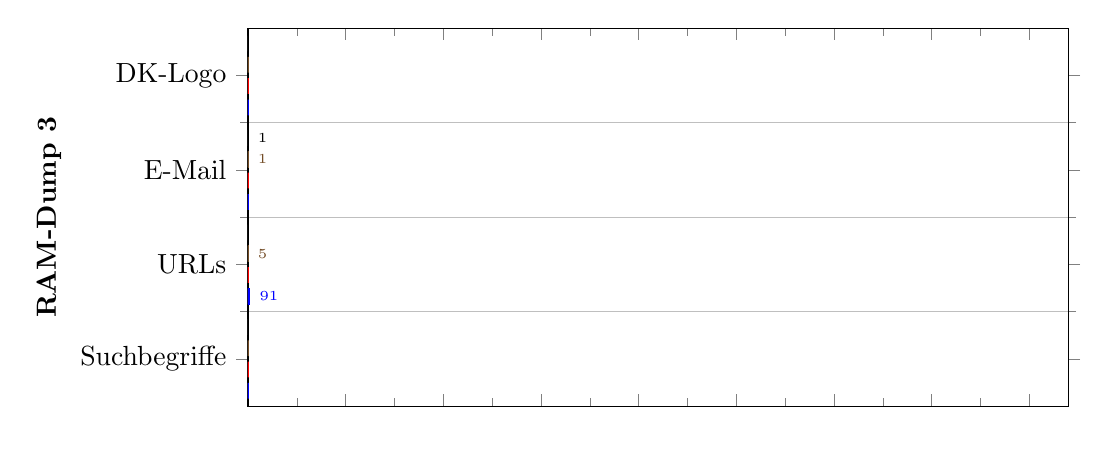
\begin{tikzpicture}
			\begin{axis}[
			xbar,
			width=12cm, 
			height=3cm, 
			ylabel style={align=center}, ylabel=\textbf{RAM-Dump 3},
			y=1.2cm,
			symbolic y coords={Suchbegriffe, URLs, E-Mail, DK-Logo},
			ytick=data,
			xticklabels={,,},
            xmin = 0,
            xmax = 42000,
			nodes near coords, 
			nodes near coords align={horizontal},
			nodes near coords style={font=\tiny},
   			nodes near coords={\pgfmathfloatifflags{\pgfplotspointmeta}{0}{}{\pgfmathprintnumber{\pgfplotspointmeta}}},
			bar width=.2cm,
			enlarge y limits={abs=3*\pgfplotbarwidth},
			scaled x ticks=false,
    		yminorgrids = true,minor tick num=1,
			legend style={
				at={(0.5,-0.1)},
				anchor=north
			},
			legend columns=4
			]
				\addplot coordinates {
				(0,Suchbegriffe) (91,URLs) (0,E-Mail) (0,DK-Logo)
				};
				\addplot coordinates {
				(0,Suchbegriffe) (0,URLs) (0,E-Mail) (0,DK-Logo)
				};
				\addplot coordinates {
				(0,Suchbegriffe) (5,URLs) (1,E-Mail) (0,DK-Logo)
				};
				\addplot coordinates {
				(0,Suchbegriffe) (0,URLs) (1,E-Mail) (0,DK-Logo)
				};
			\end{axis}
%			\legend{Firefox, Tor, Chrome, Brave}
		\end{tikzpicture}
		\\[-7pt]
		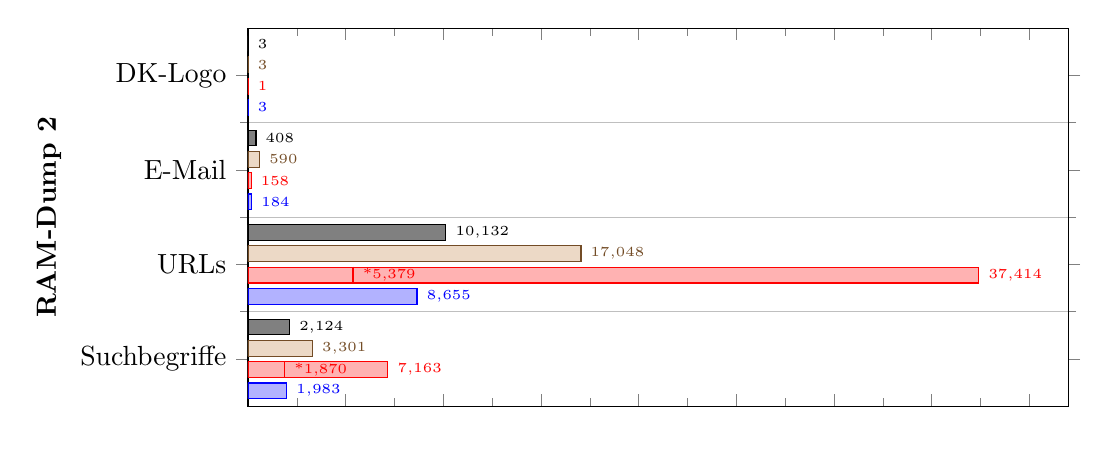
\begin{tikzpicture}
			\begin{axis}[
			xbar,
			width=12cm, 
			height=3cm, 
			ylabel style={align=center}, ylabel=\textbf{RAM-Dump 2},
			y=1.2cm,
%			symbolic y coords={Suchbegriffe, URLs, E-Mail, DK-Logo},
			ytick = {1,...,4},
			yticklabels={Suchbegriffe, URLs, E-Mail, DK-Logo},
			ytick=data,
			xticklabels={,,},
            xmin = 0,
            xmax = 42000,
			nodes near coords, 
			nodes near coords align={horizontal},
			nodes near coords style={font=\tiny},
   			nodes near coords={\pgfmathfloatifflags{\pgfplotspointmeta}{0}{}{\pgfmathprintnumber{\pgfplotspointmeta}}},
			bar width=.2cm,
			enlarge y limits={abs=3*\pgfplotbarwidth},
			scaled x ticks=false,
    		yminorgrids = true,minor tick num=1,
			legend style={
				at={(0.5,-0.1)},
				anchor=north
			},
			legend columns=4
			]
				\addplot coordinates {
				(1983,1) (8655,2) (184,3) (3,4)
				};
				\addplot coordinates {
				(7163,1) (37414,2) (158,3) (1,4)
				};
				\draw [red,line width=0.5pt] (axis cs: 5379,1.977) -- (axis cs: 5379,1.8)
				node[pos = 0.5,right] {\tiny*5,379};
				\addplot coordinates {
				(3301,1) (17048,2) (590,3) (3,4)
				};
				\draw [red,line width=0.5pt] (axis cs: 1870,0.977) -- (axis cs: 1870,0.8)
				node[pos = 0.5,right] {\tiny*1,870};
				\addplot coordinates {
				(2124,1) (10132,2) (408,3) (3,4)
				};
			\end{axis}
%			\legend{Firefox, Tor, Chrome, Brave}
		\end{tikzpicture}
		\\[-7pt]
		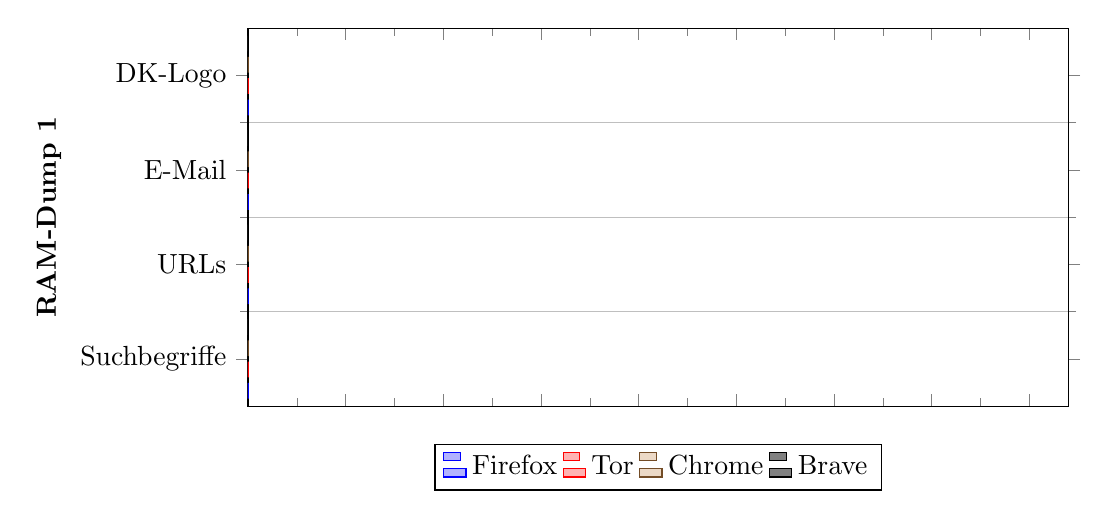
\begin{tikzpicture}
			\begin{axis}[
			xbar,
			width=12cm, 
			height=3cm, 
			ylabel style={align=center}, ylabel=\textbf{RAM-Dump 1},
			y=1.2cm,
%			symbolic y coords={Suchbegriffe, URLs, E-Mail, DK-Logo},
			ytick = {1,...,4},
			yticklabels={Suchbegriffe, URLs, E-Mail, DK-Logo},
%			ytick=data,
			xticklabels={,,},
            xmin = 0,
            xmax = 42000,
			nodes near coords, 
			nodes near coords align={horizontal},
			nodes near coords style={font=\tiny},
   			nodes near coords={\pgfmathfloatifflags{\pgfplotspointmeta}{0}{}{\pgfmathprintnumber{\pgfplotspointmeta}}},
			bar width=.2cm,
			enlarge y limits={abs=3*\pgfplotbarwidth},
			scaled x ticks=false,
    		yminorgrids = true,minor tick num=1,
			legend style={
				at={(0.5,-0.1)},
				anchor=north
			},
			legend columns=4
			]
				\addplot coordinates {
				(0,1) (0,2) (0,3) (0,4)
				};
				\addplot coordinates {
				(0,1) (0,2) (0,3) (0,4)
				};
				\addplot coordinates {
				(0,1) (0,2) (0,3) (0,4)
				};
				\addplot coordinates {
				(0,1) (0,2) (0,3) (0,4)
				};
			\legend{Firefox, Tor, Chrome, Brave}
			\end{axis}
		\end{tikzpicture}	
	\end{tabular}
	}
	\caption{Zusammenfassung gefundener Artefakte in den Firefox RAM-Dumps}
	\label{chart:firefox-volatility-summary}
\end{table}

> In keinem Browser in RAM-Dump 1 (vor dem Browsing Szenario) PB Artefakte gefunden

\paragraph*{Firefox vs Tor}
> RAM-Dump 2: 
 - Tor hinterlässt nach Browsing Szenario mit geöffnetem Browser (erstaunlicherweise) mehr URL-Artefake und Suchbegriffe im zweiten RAM-Dump als Firefox. Wert reduziert sich jedoch deutlich nach Zuweisung von "Neuer Identität" in Tor => Danach weniger Artefake in RAM hinterlassen als Firefox (Werte mit * gekennzeichnet)
 - Sowohl Tor als auch Firefox hinterlassen Gmail-Passwort als Klartext im RAM
> RAM-Dump 3:
- Nach Schließen des Browsers konnten im dritten Firefox RAM-Dump URLs im DNSCache Windows Service gefunden werden. Nach leeren des Caches und Beenden des DNSCache Services konnten wurden keine Artefakte gefunden
- Tor hinterlässt keine Artefakte nach Schließen des Browsers => .onion-URLs nicht im DNScache

=> Tor hinterlässt in RAM-2 nach Neuer Identität und in RAM-3 nach geschlossenem Browser weniger Artefakte als Firefox

\paragraph*{Chrome vs Brave}
> ... *** TODO: Christoph ***
=> Brave hinterlässt weniger Artefakte als Chrome

\paragraph*{Firefox vs Chrome}
> In RAM-Dump 2: Firefox hinterlässt in jeder Kategorie gleich viele (DK-Logo) oder weniger (E-Mail, URLs, Suchbegriffe) Artefakte als Chrome
> Durchschnittliche Differenz: 2.529 Artefakte weniger als in Chrome, größter Unterschied bei URLs
> In Ram-Dump 3: Firefox hinterlässt mehr URLs als Chrome, In Chrome zusätzlich 1x Absender-Adresse gefunden.

\paragraph*{Tor vs Brave}
> Vor "Neuer Identität" hinterlässt Tor deutlich mehr URL- und Suchbegriff-Artefakte als Brave
	=> Insbesondere hinterlässt Tor 2x das Gmail-Passwort als Klartext im RAM
> Nach "Neuer Identiät" hinterlässt Tor in RAM-Dump 2 weniger Artefakte als Brave (Durchschnittliche Differenz = 1315 Artefakte weniger als Brave), wobei größter Unterschied bei URLs, Passwort nicht mehr im RAM

> In RAM-Dump 3 hinterlässt Tor kein Artefakt, Brave 1x die Absender-Mail
















